\section{Caching}

\paragraph{Caching --- Motivation}
\begin{itemize}
  \item memory (RAM) needs to be managed carefully
  \item \textbf{Ideal} properties: large, fast, nonvolatile, cheap
  \item \textbf{Real} memory: trade-offs
\end{itemize}

\paragraph{Caching --- Cache misses}
\begin{itemize}
  \item \textbf{Compulsory miss}:
  \begin{itemize}
    \item cold start, first reference
    \item data block was not cached before
  \end{itemize}
  \item \textbf{Capacity miss}:
  \begin{itemize}
    \item not all required data fits into cache
    \item accessed data previously evicted to make room for different data
  \end{itemize}
  \item \textbf{Conflict miss}:
  \begin{itemize}
    \item collision, interference
    \item depending on cache organization, data items interfere with each other
    \item fully associative caches are not prone to conflict misses
  \end{itemize}
\end{itemize}

\paragraph{Caching --- Harvard architecture}
\begin{itemize}
  \item \textbf{Principle}: separate buffer memory for data and instructions
\end{itemize}
\begin{figure}[h]\centering\label{CachingHarvard}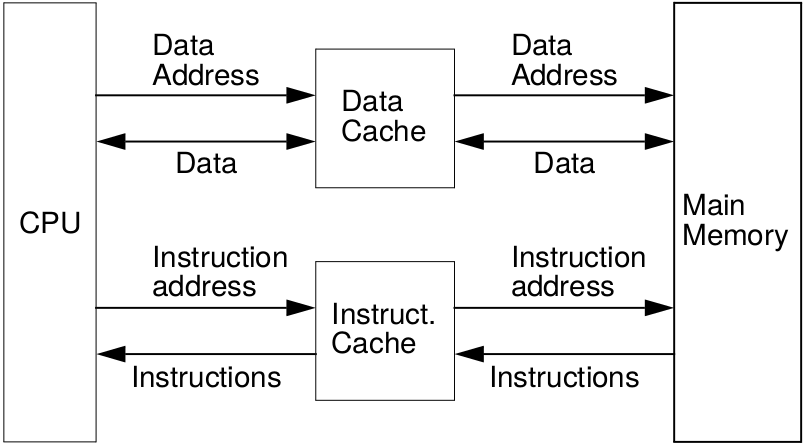
\includegraphics[width=0.33\textwidth]{CachingHarvard}\end{figure}

\paragraph{Caching --- write/replacement policies}
\begin{itemize}
  \item \textbf{Cache hit}:
  \begin{itemize}
    \item \emph{write-through}: main memory always up-to-date, writes might be slow
    \item \emph{write-back}: data written only to cache, main memory temporarily inconsistent
  \end{itemize}
  \item \textbf{Cache miss}:
  \begin{itemize}
    \item \emph{write-allocate}: data read from main memory to cache, write performed afterwards
    \item \emph{write-to-memory}: modification is performed only in main memory
  \end{itemize}
\end{itemize}

\paragraph{Cache Design Parameters}
\begin{itemize}
  \item \textbf{Size + Set size}: small cache $ \to $ set-associative implementation with large sets
  \item \textbf{Line length}: spatial locality $ \to $ long cache lines
  \item \textbf{Write policy}: temporal locality $ \to $ write-back
  \item \textbf{Replacement policy}
  \item \textbf{Tagging/Indexing}: virtual or physical addresses
\end{itemize}

\paragraph{Caching --- Problems}
\begin{itemize}
  \item \textbf{Ambiguity problem}: same virtual addresses point to different physical addresses at different times
  \item \textbf{Alias problem}: different virtual addresses point to same physical memory location
\end{itemize}

\paragraph{Caching --- virtually indexed, virtually tagged}
\begin{itemize}
  \item \textbf{Operations}:
  \begin{itemize}
    \item \emph{context switch}: cache must be invalidated (and written back if write-back is used)
    \item \emph{fork}: child needs complete copy of parent's address space
    \item \emph{exec}: invalidate cache, no write-back necessary
    \item \emph{exit}: flush cache
    \item \emph{brk/sbrk}: growing = nothing, shrinking = (selective) cache invalidations
  \end{itemize}
  \item \textbf{shared memory/memory-mapped files}: alias problem!
  \begin{itemize}
    \item disallow, do not cache
    \item only allow addresses mapping to same cache line (if using direct-mapped write-allocate cache)
    \item each frame accessible from exactly one virtual address at any time $ \to $ alias page invalidation
  \end{itemize}
  \item \textbf{I/O}:
  \begin{itemize}
    \item \emph{buffered I/O}: no problems 
    \item \emph{unbuffered I/O}:
    \begin{itemize}
      \item write: information may still be in cache $ \to $ write back before I/O starts
      \item read: cache must be invalidated
    \end{itemize}
  \end{itemize}
\end{itemize}
\begin{figure}[h]\centering\label{VIVT}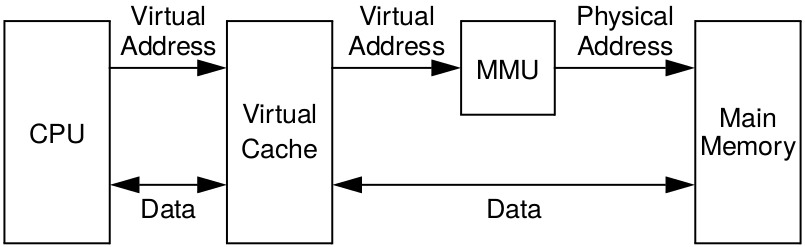
\includegraphics[width=0.33\textwidth]{VIVT}\end{figure}

\paragraph{Caching --- virtually indexed, physically tagged}
\begin{itemize}
  \item \textbf{Usage}: often used as first-level cache
  \item \textbf{Management}:
  \begin{itemize}
    \item no ambiguities
    \item no cache flush on context switch
    \item shared memory/memory mapped files: virtual starting addresses must be mapped to same cache line
    \item I/O: cache flush required
  \end{itemize}
  \item \textbf{Conflicts}: data structures with address distance = multiple of cache size are mapped to same line
  \item \textbf{Runtime properties}:
  \begin{itemize}
    \item \emph{cache flush}: avoidable most times (fast context switches, interrupt-handling, syscalls)
    \item \emph{deferred write-back after context switch}:
    \begin{itemize}
      \item avoids write accesses $ \to $ performance gain
      \item variable execution time caused by compulsory misses
    \end{itemize}
    \item \emph{dynamic memory management}: causes variable execution times through conflict misses
    \item \emph{multiprocessor systems}: problematic with shared memory --- which line should be invalidated?
    \begin{itemize}
      \item cache size is small multiple of page size (1-4)
      \item requires to only invalidate/flush 1-4 cache lines by cache coherency HW
    \end{itemize}
  \end{itemize}
\end{itemize}
\begin{figure}[h]\centering\label{VIPT}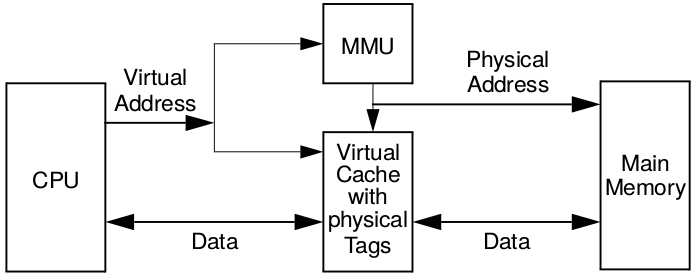
\includegraphics[width=0.33\textwidth]{VIPT}\end{figure}

\paragraph{Caching --- physically indexed, physically tagged}
\begin{itemize}
  \item \textbf{Advantages}:
  \begin{itemize}
    \item[+] completely transparent to processor
    \item[+] no performance-critical system support required (including I/O)
    \item[+] SMPs with shared memory can use coherency protocol implemented in hardware
  \end{itemize}
  \item \textbf{random allocation conflicts}:
  \begin{itemize}
    \item page conflicts caused by random allocation of physical memory
    \item contiguous virtual memory normally mapped to arbitrary free physical pages
  \end{itemize}
  \item \textbf{random coloring conflicts}: consequences of random page coloring:
  \begin{itemize}
    \item cache conflicts
    \item cache only partially used
    \item significant runtime variations
  \end{itemize}
  \item \textbf{conflict mitigation}:
  \begin{itemize}
    \item sequential page colors for individual memory segments
    \item \emph{cache partitioning}: divide physical memory in disjoint subsets, all pages of subset are mapped to same cache partition
  \end{itemize}
\end{itemize}
\begin{figure}[h]\centering\label{PIPT}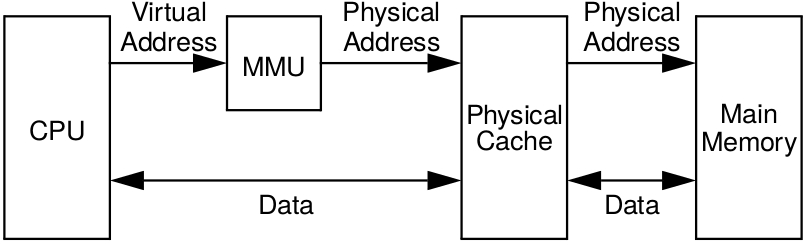
\includegraphics[width=0.33\textwidth]{PIPT}\end{figure}
